\documentclass{article}
\usepackage{graphicx} % Required for inserting images
\usepackage{amsmath}
\usepackage{mathtools}
\usepackage{amssymb}
\usepackage{xparse}
\usepackage{physics}
\usepackage{esint}
\usepackage{enumitem}
\usepackage{mathptmx}
\usepackage{graphicx}
\usepackage{float}

\title{CTA200 - Assignment3}
\author{Brian Huang}
\date{May 2026}

\begin{document}

\maketitle

\section*{Introduction}
In this assignment, I studied two examples of nonlinear systems using numerical methods. Firstly, I computed the Mandelbrot set by iterating a complex equation over a grid of points on the complex plane. Secondly, I solve the Lorenz system equations, which are 3 coupled nonlinear ordinary differential equation. The goal for this assignment was to visualize bounded and divergent behaviours in Mandelbrot set, and to investigate chaotic behaviour among Lorenz system.

\section*{Question 1: Mandelbrot Set}
For the Mandelbrot set, I consider the complex number in the form of $c = x + iy$, where $-2<x<2$ and $-2< y < 2$. For each $c$, I started with $z_0 = 0$ and iterated:
\begin{equation}
    z_{n+1} = z_n^2 + c.
\end{equation}
I classified the point that is diverged if the magnitude $\abs{z}$ after the iteration became larger than 2 before reaching the maximum number of iterations. On the other hand, the point is bounded if it stay inside or on the boundary after reaching the maximum number of iterations.
\begin{figure}
    \centering
    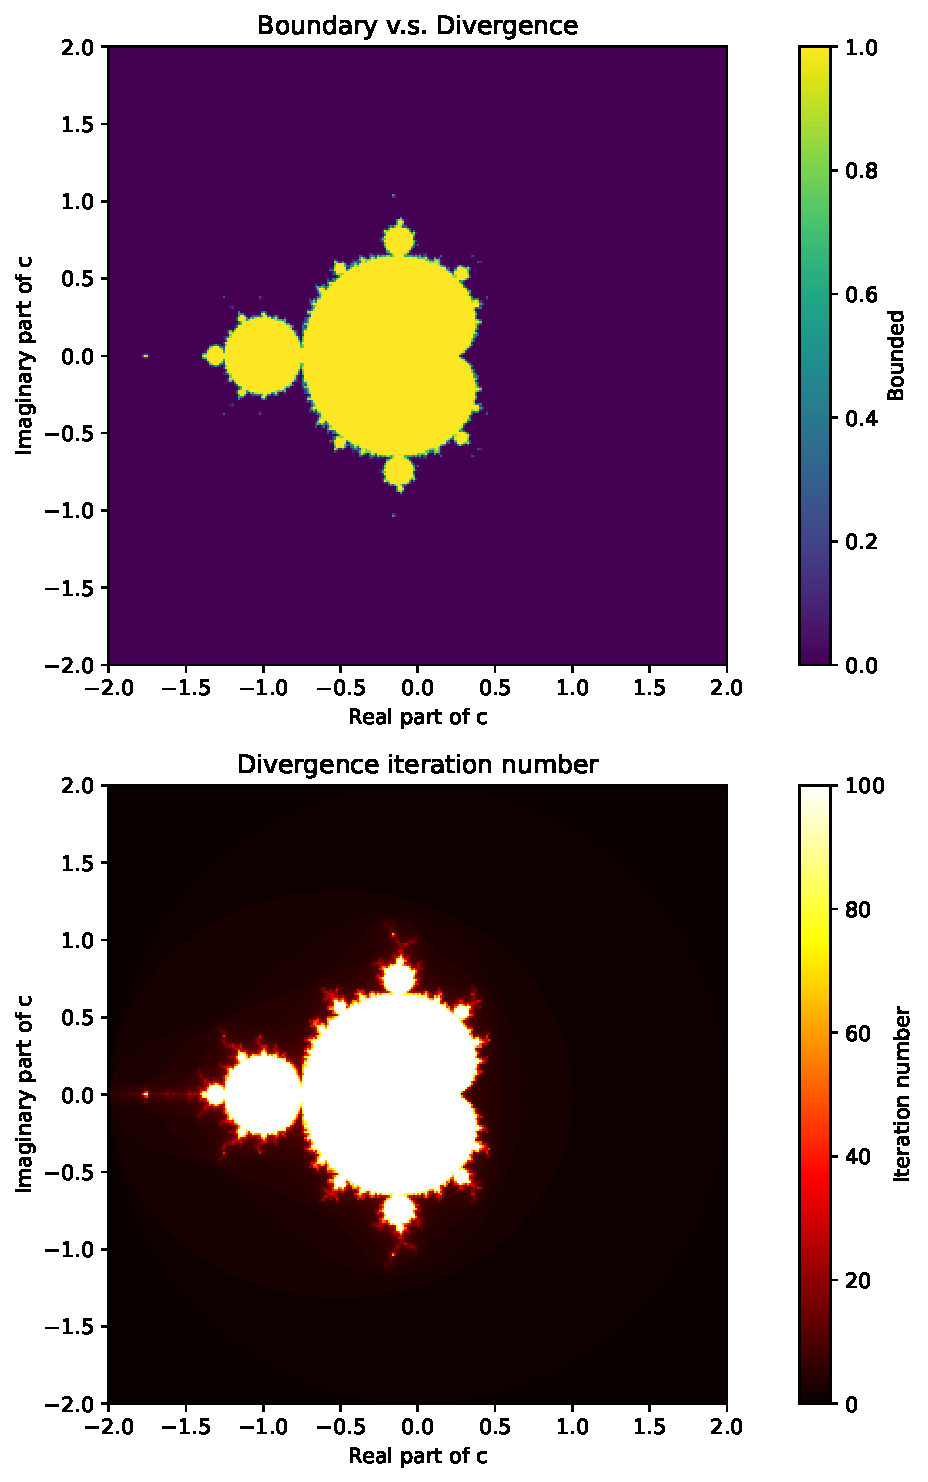
\includegraphics[width=0.95\linewidth]{figure1_mandelbrot.pdf}
    \caption{Mandelbrot set and divergence iteration number}
    \label{fig:mandelbrot}
\end{figure}
The top panel of the figure \ref{fig:mandelbrot} shows the bounded and divergent region in the complex plane. The bottom one shows the iteration number that each point diverges, the points in the bounded region all has the maximum iteration number. Through the high contract colour map, we can see the points near the boundary of the Mandelbrot set usually tend to take longer to diverge. Therefore, those points creates a clear structure around the edge of the set.

\section*{Question 2}
For the Lorenz system, I solved the equations:
\begin{align}
    \dot{X} &= -\sigma(X - Y) \\[6pt]
    \dot{Y} &= rX - Y - XZ \\[6pt]
    \dot{Z} &= -bZ + XY.
\end{align}
With the initial condition given by the question, $W_0 = [0,\ 1,\ 0]$, and the parameter $\sigma = 10$, $r = 28$, and $b = 8/3$, we solved the system using function "solve\_\ ivp" from scipy.integrate package and integrated from $t = 0$ to $t = 60$. 
To reproduce Lorenz's figure 1, I plotted $Y$ as a function of the iteration number $N = t/\Delta t$, where $\Delta t=0.01$.
\begin{figure}
    \centering
    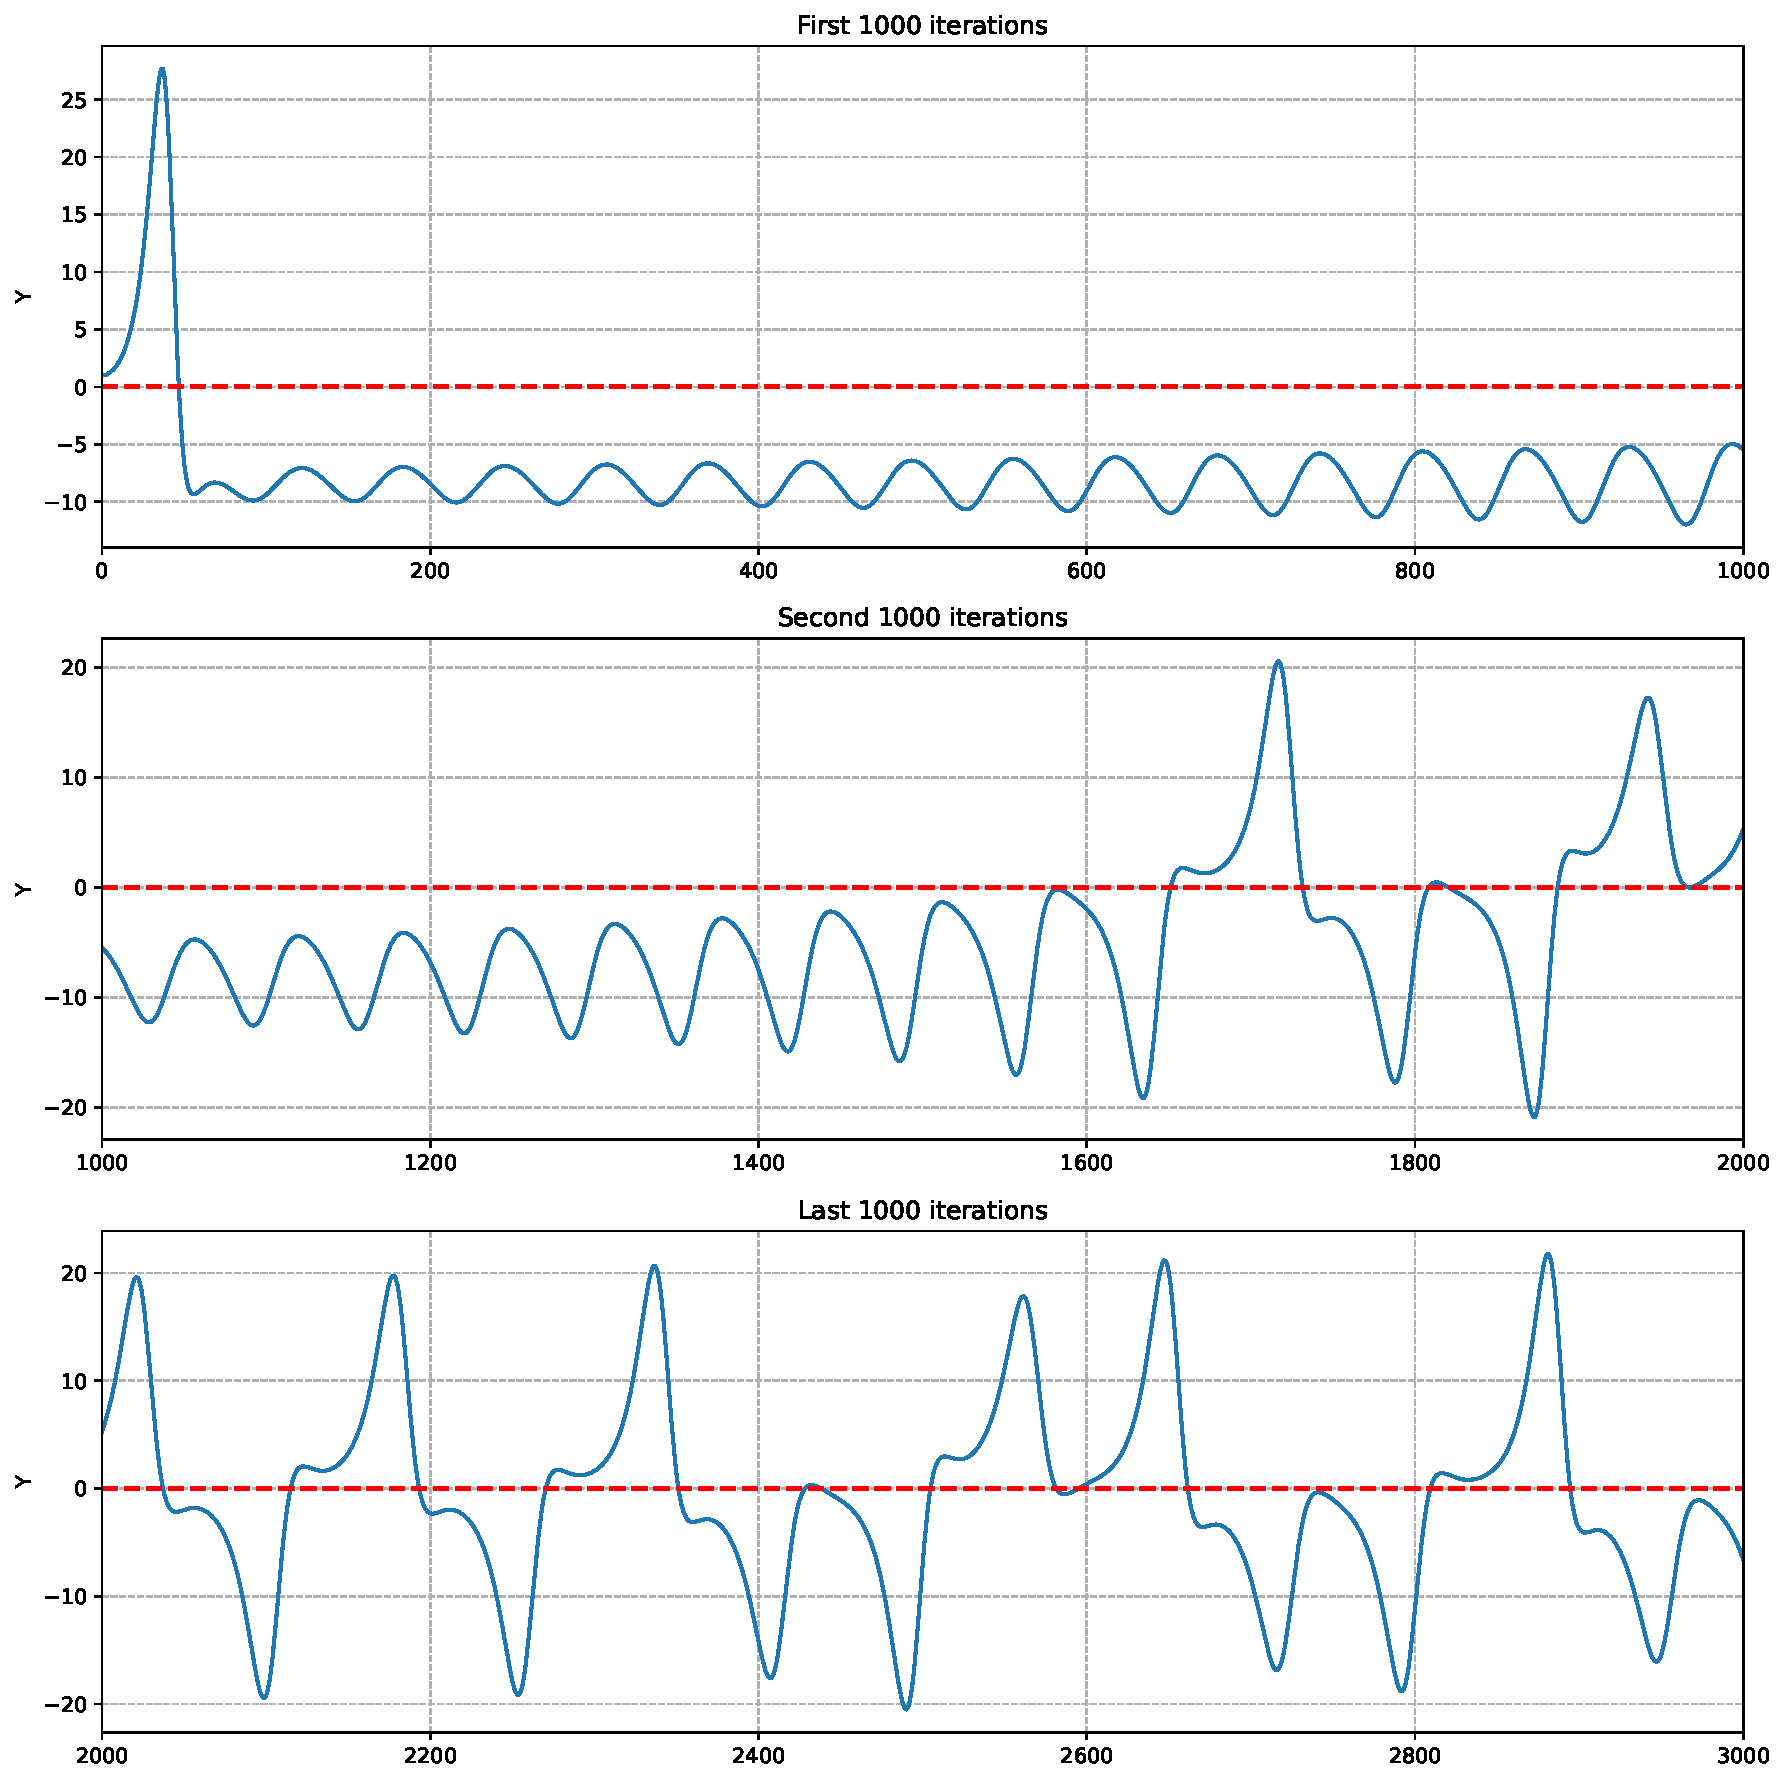
\includegraphics[width=1\linewidth]{figure2_lorenz_fig1.pdf}
    \caption{Reproduction of Lorenz Figure 1. Top: First 1000 iterations; Middle: Second 1000 iterations; Bottom: Third 1000 iterations.}
    \label{fig:lorenz_fig1}
\end{figure}
From our reproduced figure \ref{fig:lorenz_fig1}, we can see the solution begins with a transient spike then develop an irregular oscillating features, which means the system was adjusting from the given initial condition, and the irregular oscillating patterns show the chaotic behaviour of the Lorenz's system. Compare to Lorenz's figure 1, our reproduction has the same pattern as Lorenz's figure 1, in which particularly the first cross-zero spike around iteration 1600 but closer to 1700 in Lorenz's figure 1. This small mismatch is expected, because the Lorenz system is chaotic and any small numerical difference between our solver and Lorenz's original method will grow over time, so the two trajectories cannot stay identical. Therefore, you will see the pattern looks completely mismatched after the first cross-zero spike to iteration 3000. I also reproduced Lorenz's Figure 2 by plotting the trajectory from $t=14$ to $t=19$, corresponding to iterations 1400 to 1900. Figure \ref{fig:lorenz_fig2} shows projections of the trajectory onto the $Y$-$Z$ and $Y$-$X$ planes. These phase-space projections show that the motion does not settle into a simple periodic orbit. Comparing to Lorenz's original figure 2 with our reproductions, these two projections of trajectory onto different planes look identical. 
Finally, I solved the Lorenz equations against a slightly perturbed initial conditions:
\begin{equation}
    W_0' = [0,\ 1.00000001,\ 0].
\end{equation}
I then calculated the distance between the original and perturbed solutions:
\begin{equation}
    d(t) = \sqrt{
    (X_1-X_2)^2 + (Y_1-Y_2)^2 + (Z_1-Z_2)^2
    }.
\end{equation}
Figure \ref{fig:perturbation} shows this distance on a semi-log plot, with linear time and logarithmic distance. The distance grows rapidly over time, showing that a very small difference in the initial condition can lead to a large difference in the later solution.
\begin{figure}
    \centering
    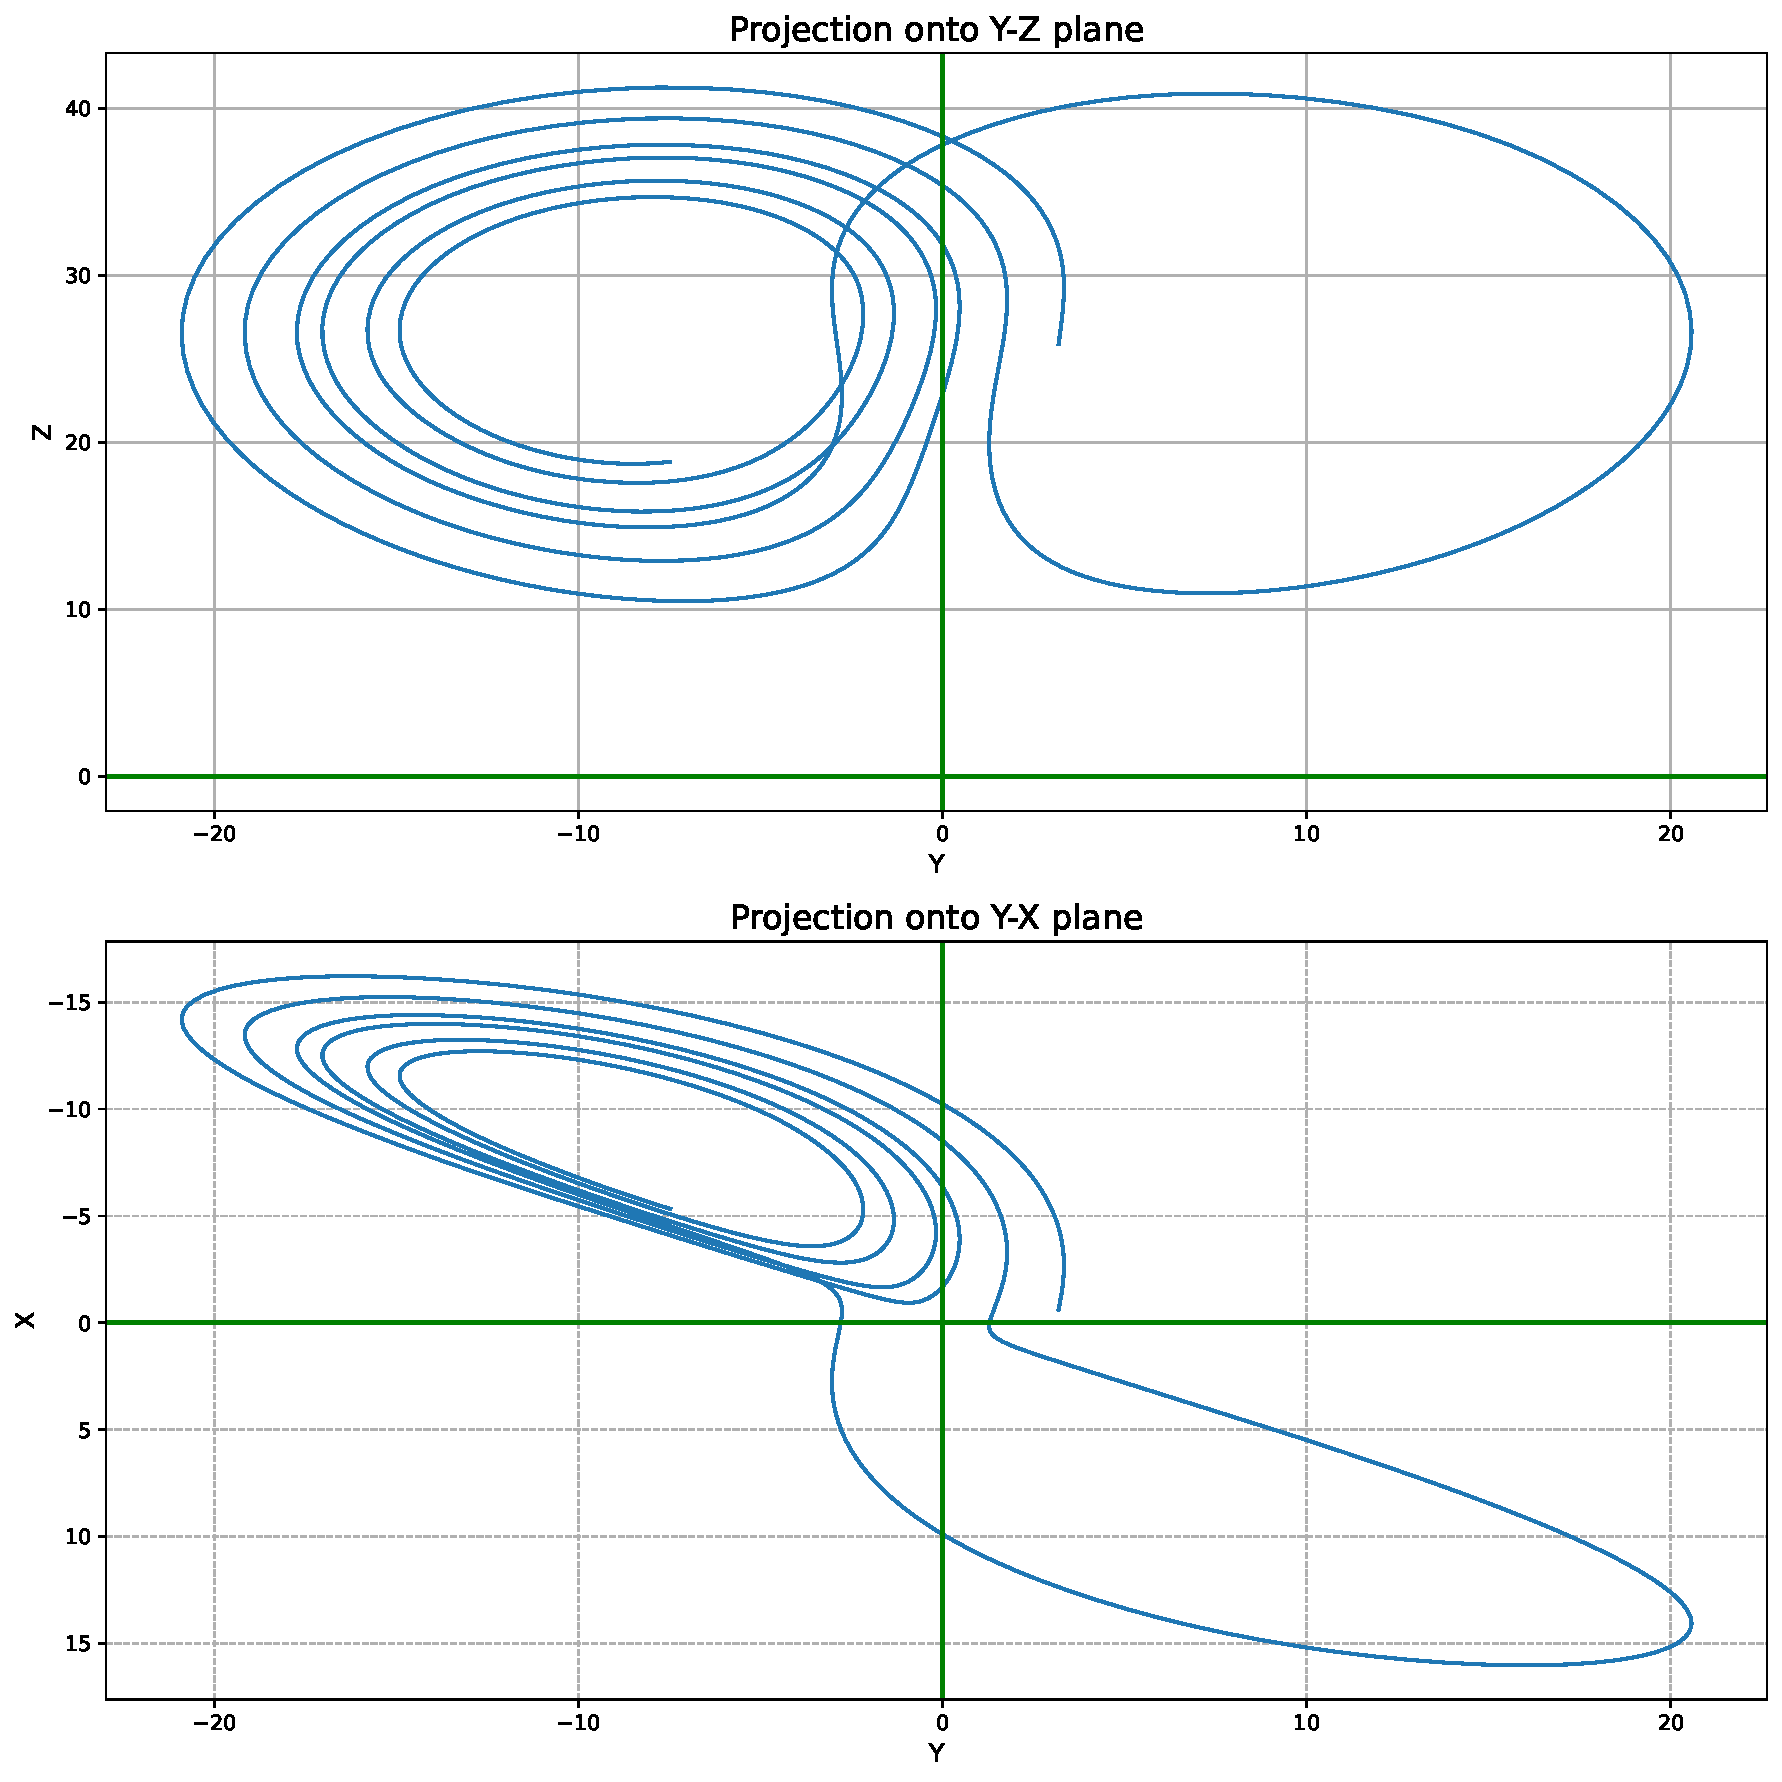
\includegraphics[width=1\linewidth]{figure3_lorenz_fig2.pdf}
    \caption{Reproduction of Lorenz Figure 2. Top: Projection on Y-Z plane; Bottom: Projection on Y-X
    plane with inverted axes.}
    \label{fig:lorenz_fig2}
\end{figure}

\begin{figure}
    \centering
    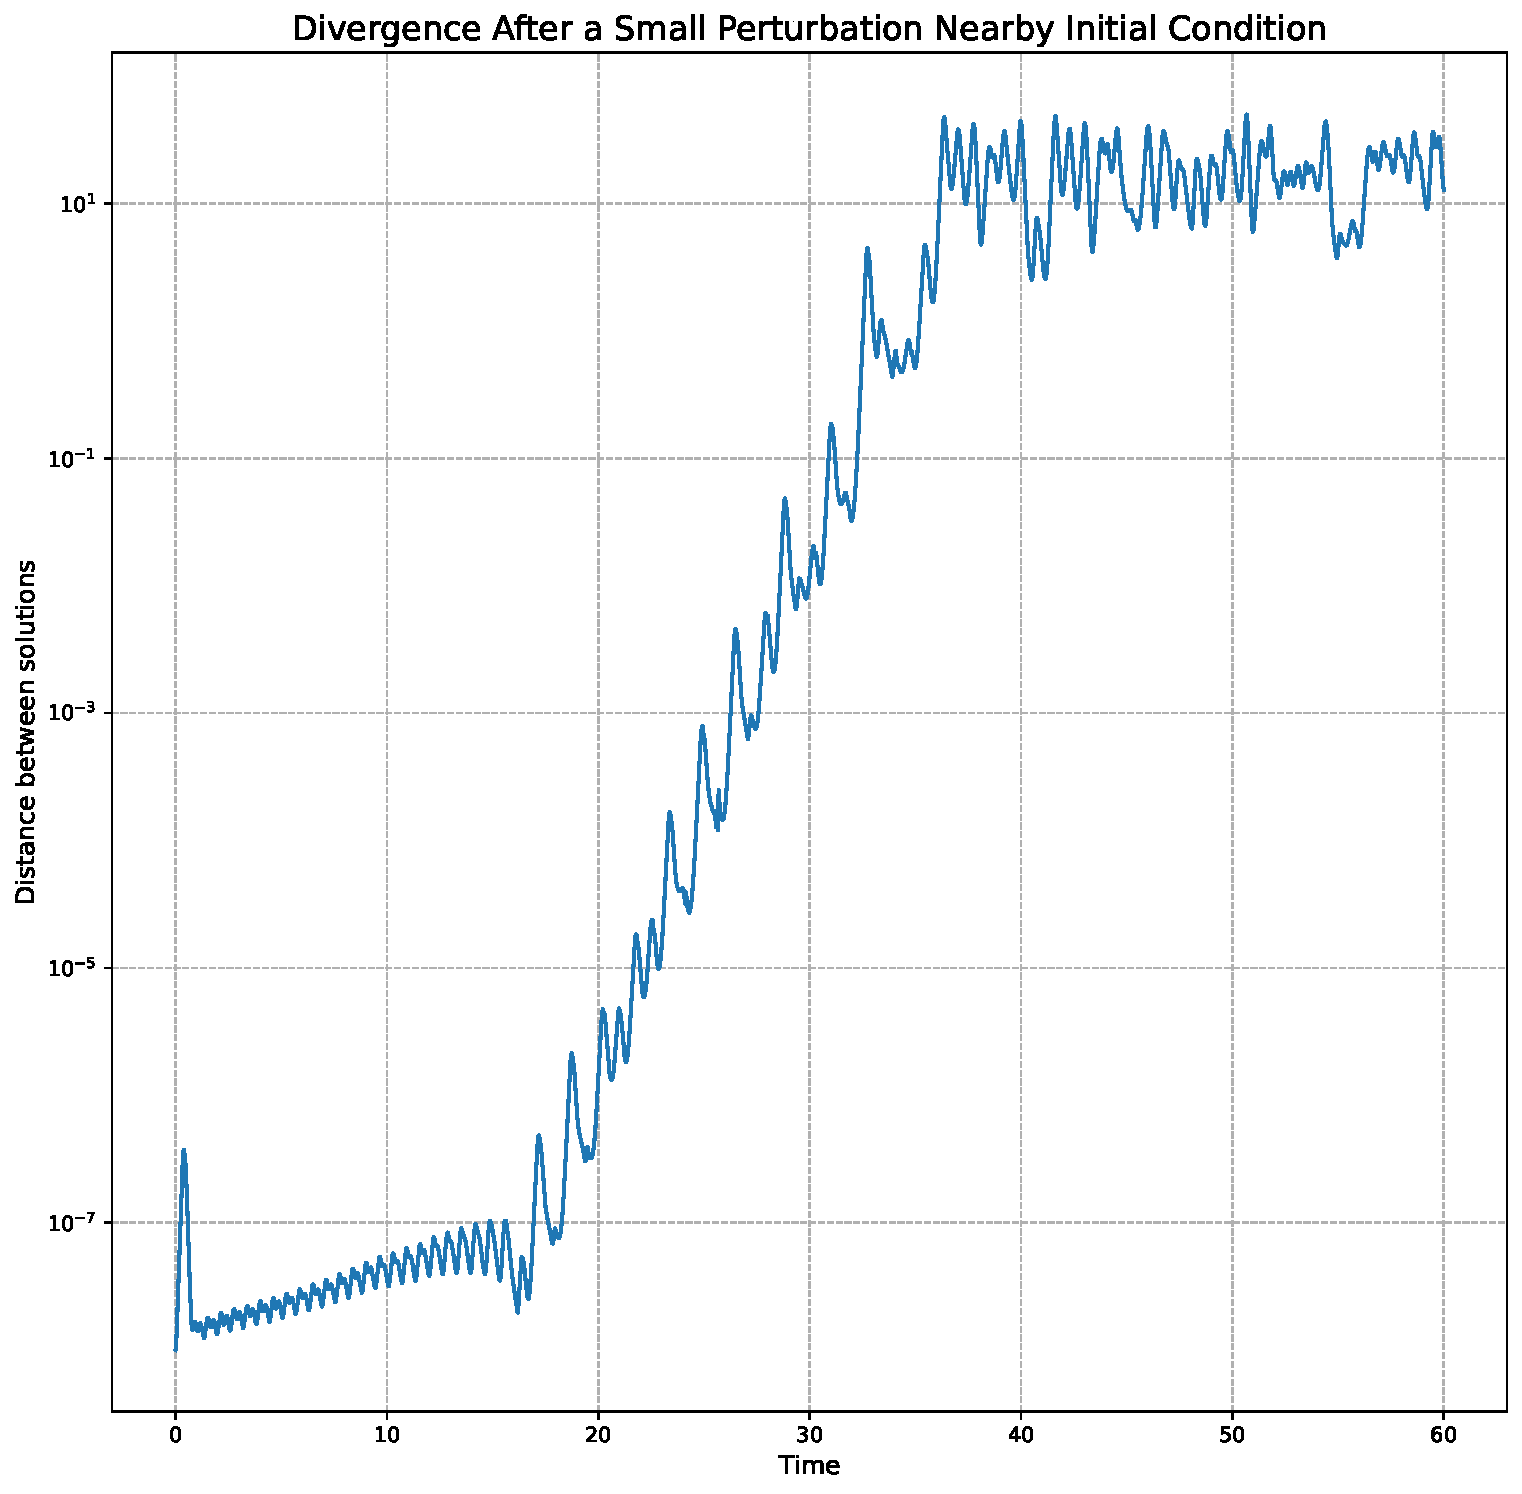
\includegraphics[width=1\linewidth]{figure4_perturbation.pdf}
    \caption{Perturbation distance semi-log plot as a function of time, x-axis: linear time; y-axis: logarithmic distance.}
    \label{fig:perturbation}
\end{figure}

\section*{Conclusion}
The Mandelbrot set and the Lorenz equations both demonstrate how simple nonlinear rules can produce complex behaviour. For the Mandelbrot set, different complex values of $c$ led either to bounded or divergent sequences, with the most detailed structure appearing near the boundary. For the Lorenz system, the numerical solution showed irregular oscillations and strong sensitivity to initial conditions. The slight perturbation to the initial conditions showed that two solutions starting extremely close together can separate quickly, which is a key feature of chaotic systems.
\end{document}
